% \section{Versions séquentielles}
% \subsection{Considérations}
% Le code est exécuté sur un coeur d'un Intel Xeon E5-2680 v3 @ 2.50GHz d'un noeud miriel de Plafrim.\\
% C'est une architecture Haswell, capable de réaliser 16 opérations flottantes par cycle par coeur, avec une vitesse d'horloge maximale de 2.5Ghz, donnant un maximum théorique de 40 GFlop/s sur un seul coeur.
% \subsection{Implémentation du produit scalaire}
% Nous avons implémentés une version naïve du produit scalaire, parcourant deux vecteurs pour calculer $<a,b>=\sum_{i=1}^n{a_ib_i}$ pour $a$ et $b$ dans $\mathbb{K}^n$. Comme nous ne l'utiliserons pas dans notre DGEMM, nous n'allons pas perdre de temps à essayer de l'optimiser. De plus, chaque valeur n'étant utilisée qu'une et une seule fois nous ne voyons pas de stratégies d'optimisation évidente.\\
% Voici une comparaisons sur des vecteurs de tailles croissante entre notre implémentation et celle d'OpenBLAS:
% \begin{figure}[H]
%     \centering
%     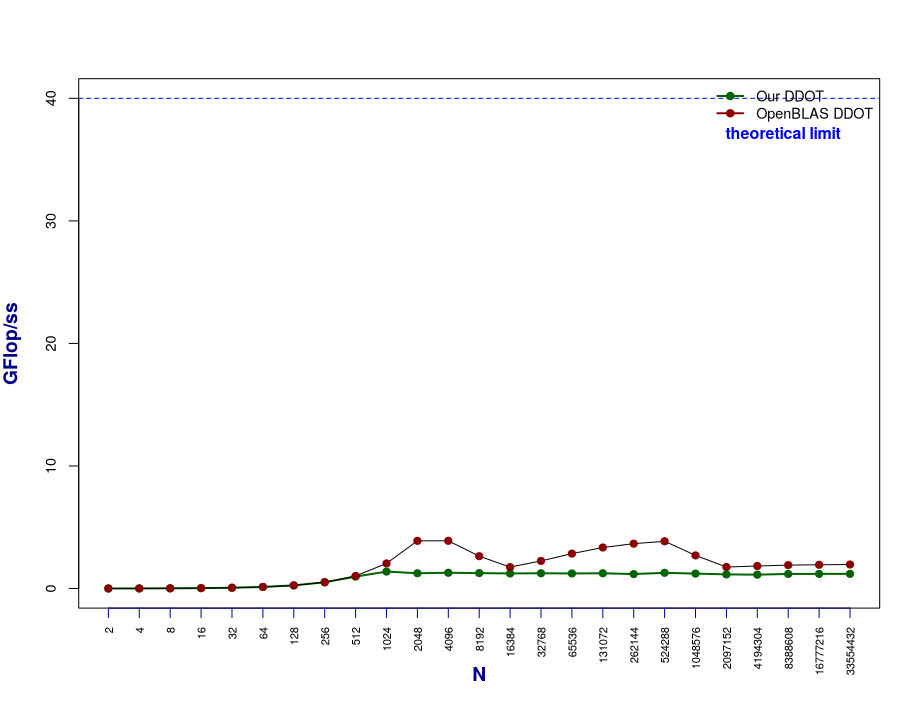
\includegraphics[width=0.925\linewidth]{assets/ddot_seq_vs_vendor.png}
%     \caption{Comparaison entre l'implémentation du produit scalaire d'OpenBLAS et la notre.}
%     \label{fig:placeholder}
% \end{figure}
% On constate donc que, même avec un kernel optimisé, OpenBLAS n'est plus performant que notre implémentation uniquement sur de grands vecteurs ($N > 512$), et que le gain n'est pas significatif car nous restons bien loin du pic théorique. C'est attendu étant donné que; comme dit précédemment, chaque donnée est utilisée une et une seule fois. Cela implique un grand nombre d'aller-retour en mémoire pour une intensité arithmétique faible, un très mauvais cas de figure donc pour maximiser l'utilisation d'un processeur !

% \subsection{Implémentation du produit matriciel}
% Nous nous baserons, à minima pour les versions CPU du produit matriciel sur l'implémentation classique à trois boucles (en suivant l'ordre $n, k, m$) pour le cas où A et B ne sont pas transposées. Nous réaliserons l'opération $\alpha AB+\beta C$, en prenant donc en compte les valeurs de $\alpha$ et $\beta$. Nous reviendrons sur les performances de cette implémentation plus tard afin de ne pas surcharger le rapport de figures peu intéressantes. Il sera présenté sour le nom de kernel "scalaire". C'est le kernel fourni de base dans le code. Nous avons décidé de le garder car notre implémentation était très similaire, ne gérant simplement pas les cas impliquants une matrice transposée.
% \subsection{Implémentation de la factorisation LU}
% <TODO>

% \section{Blocage et vectorisation}
% \subsection{Implémentatin d'une version en blocs}
% Nous avons implémentés une version en blocs se reposant sur le kernel de DGEMM "scalaire". Cette dernière est assez simple, nous avons reprit le code du kernel "scalaire", et avons ajoutés un pas égal à `dgemm\_seq\_bloc\_size`. Pour tous les blocs nous allons d'abord appeler scale\_bloc\` pour multiplier les valeurs de $C$ par $\beta$, puis nous appelons le kernel scalaire sur le bloc courant. L'implémentation est peu performante, mais nous n'avons pas cherchés à l'optimiser outre mesure car nous avons basés notre DGEMM séquentiel final sur une approche bloquée assez différente de celle-ci. Nous reviendrons également sur les performances de ce kernel plus tard dans le rapport !

% \subsection{Implémentation d'une version vectorisée}
% Comme vu précédemment, nous travaillons sur des processeurs Xeon E5-2680 v3 basés sur l'architecture Haswell. Il supporte donc entre autre les extensions SIMD AVX2 et FMA. Concrètement, nous pouvons manipuler des vecteurs de 256 bits. Un double étant un mot de 64 bits, nous pouvons donc manipuler des vecteurs de 4 doubles.\\
% Une implémentation naïve de l'opération DGEMM peut donc être faite en itérant dans la boucle interne avec un pas de 4 au lieu de 1, et en vectorisant les opérations de la boucle itérant le plus rapidement. Comme dit précédemment, nous itérons dans l'ordre $n, k, m$. Nous traiterons donc les éléments de 4 lignes consécutives à la fois pour chaque itération.\\
% Le procédé reste donc le même:\\
% Pour chaque vecteur d'une colonne $n$ de $C$, nous multiplions d'abord les $m$ éléments de ce vecteur par $\beta$, en procédant 4 lignes à la fois. Nous passons ensuite à la réduction sur la dimension $k$. Nous chargeons la valeur de $B$ correspondant au couple $n, k$ courant puis la broadcastons dans un vecteur. Ensuite, nous chargeons 4 lignes du vecteur courant de $A$ et de $C$ et ajoutons aux lignes de $C$ les valeurs des lignes de $A$ multipliées par la valeur broadcastée de $B$, en prenant en compte la multiplication par $\alpha$.\\
% Finalement, un retour en séquentiel permet de traiter les éléments finaux si $m$ n'est pas divisible par 4.\\
% \subsubsection{Impact de l'utilisation de FMA}
% L'implémentation naïve AVX2 utilise ces instruction: "C\_mn\_subvec = \_mm256\_add\_pd(C\_mn\_subvec, \_mm256\_mul\_pd(A\_mk\_subvec, B\_nk\_vec));", qui peuvent être remplacées par "C\_mn\_subvec = \_mm256\_fmadd\_pd(A\_mk\_subvec, B\_nk\_vec, C\_mn\_subvec);". En effet, le jeu d'instruction AVX2+FMA offre la possibilité de réaliser deux opérations Fuse-Multiply-Add par cycle. Cette opération permet de réaliser dans notre cas l'opération $C += A*B$. Voici comment FMA impact la rapidité du kernel:
% Nous aurions pu nous attendre à ce que le compileur optimise l'enchaînement de la multiplication et l'addition par un FMA, à minima à un niveau d'optimisation -O3, mais après une rapide lecture du code assembleur généré (en passant par Godbolt), nous constatons que ce n'est pas le cas:
% \begin{lstlisting}
% dgemm_kernel_avx2_fma:
%     (...)
%     vfmadd213pd     ymm7, ymm6, ymmword ptr [r10 + 8*rax]
%     (...)
% dgemm_kernel_avx2_nofma:
%     (...)
%     vmulpd  ymm7, ymm6, ymm7
%     vaddpd  ymm7, ymm7, ymmword ptr [r10 + 8*rax]
%     (...)
% \end{lstlisting}
% Et pourtant aucun speedup significatif n'est observé, les résultats sont les même sauf pour de très petites matrices mais ce n'est pas significatif.
% \subsubsection{Blocage + vectorisation}
% Finalement, nous pouvons remplacer l'appel à dgemm\_scalaire par un appel à dgemm\_avx2 dans la fonction dgemm\_bloc, ce qui nous donne ces résultats:
% \begin{figure}[H]
%     \centering
%     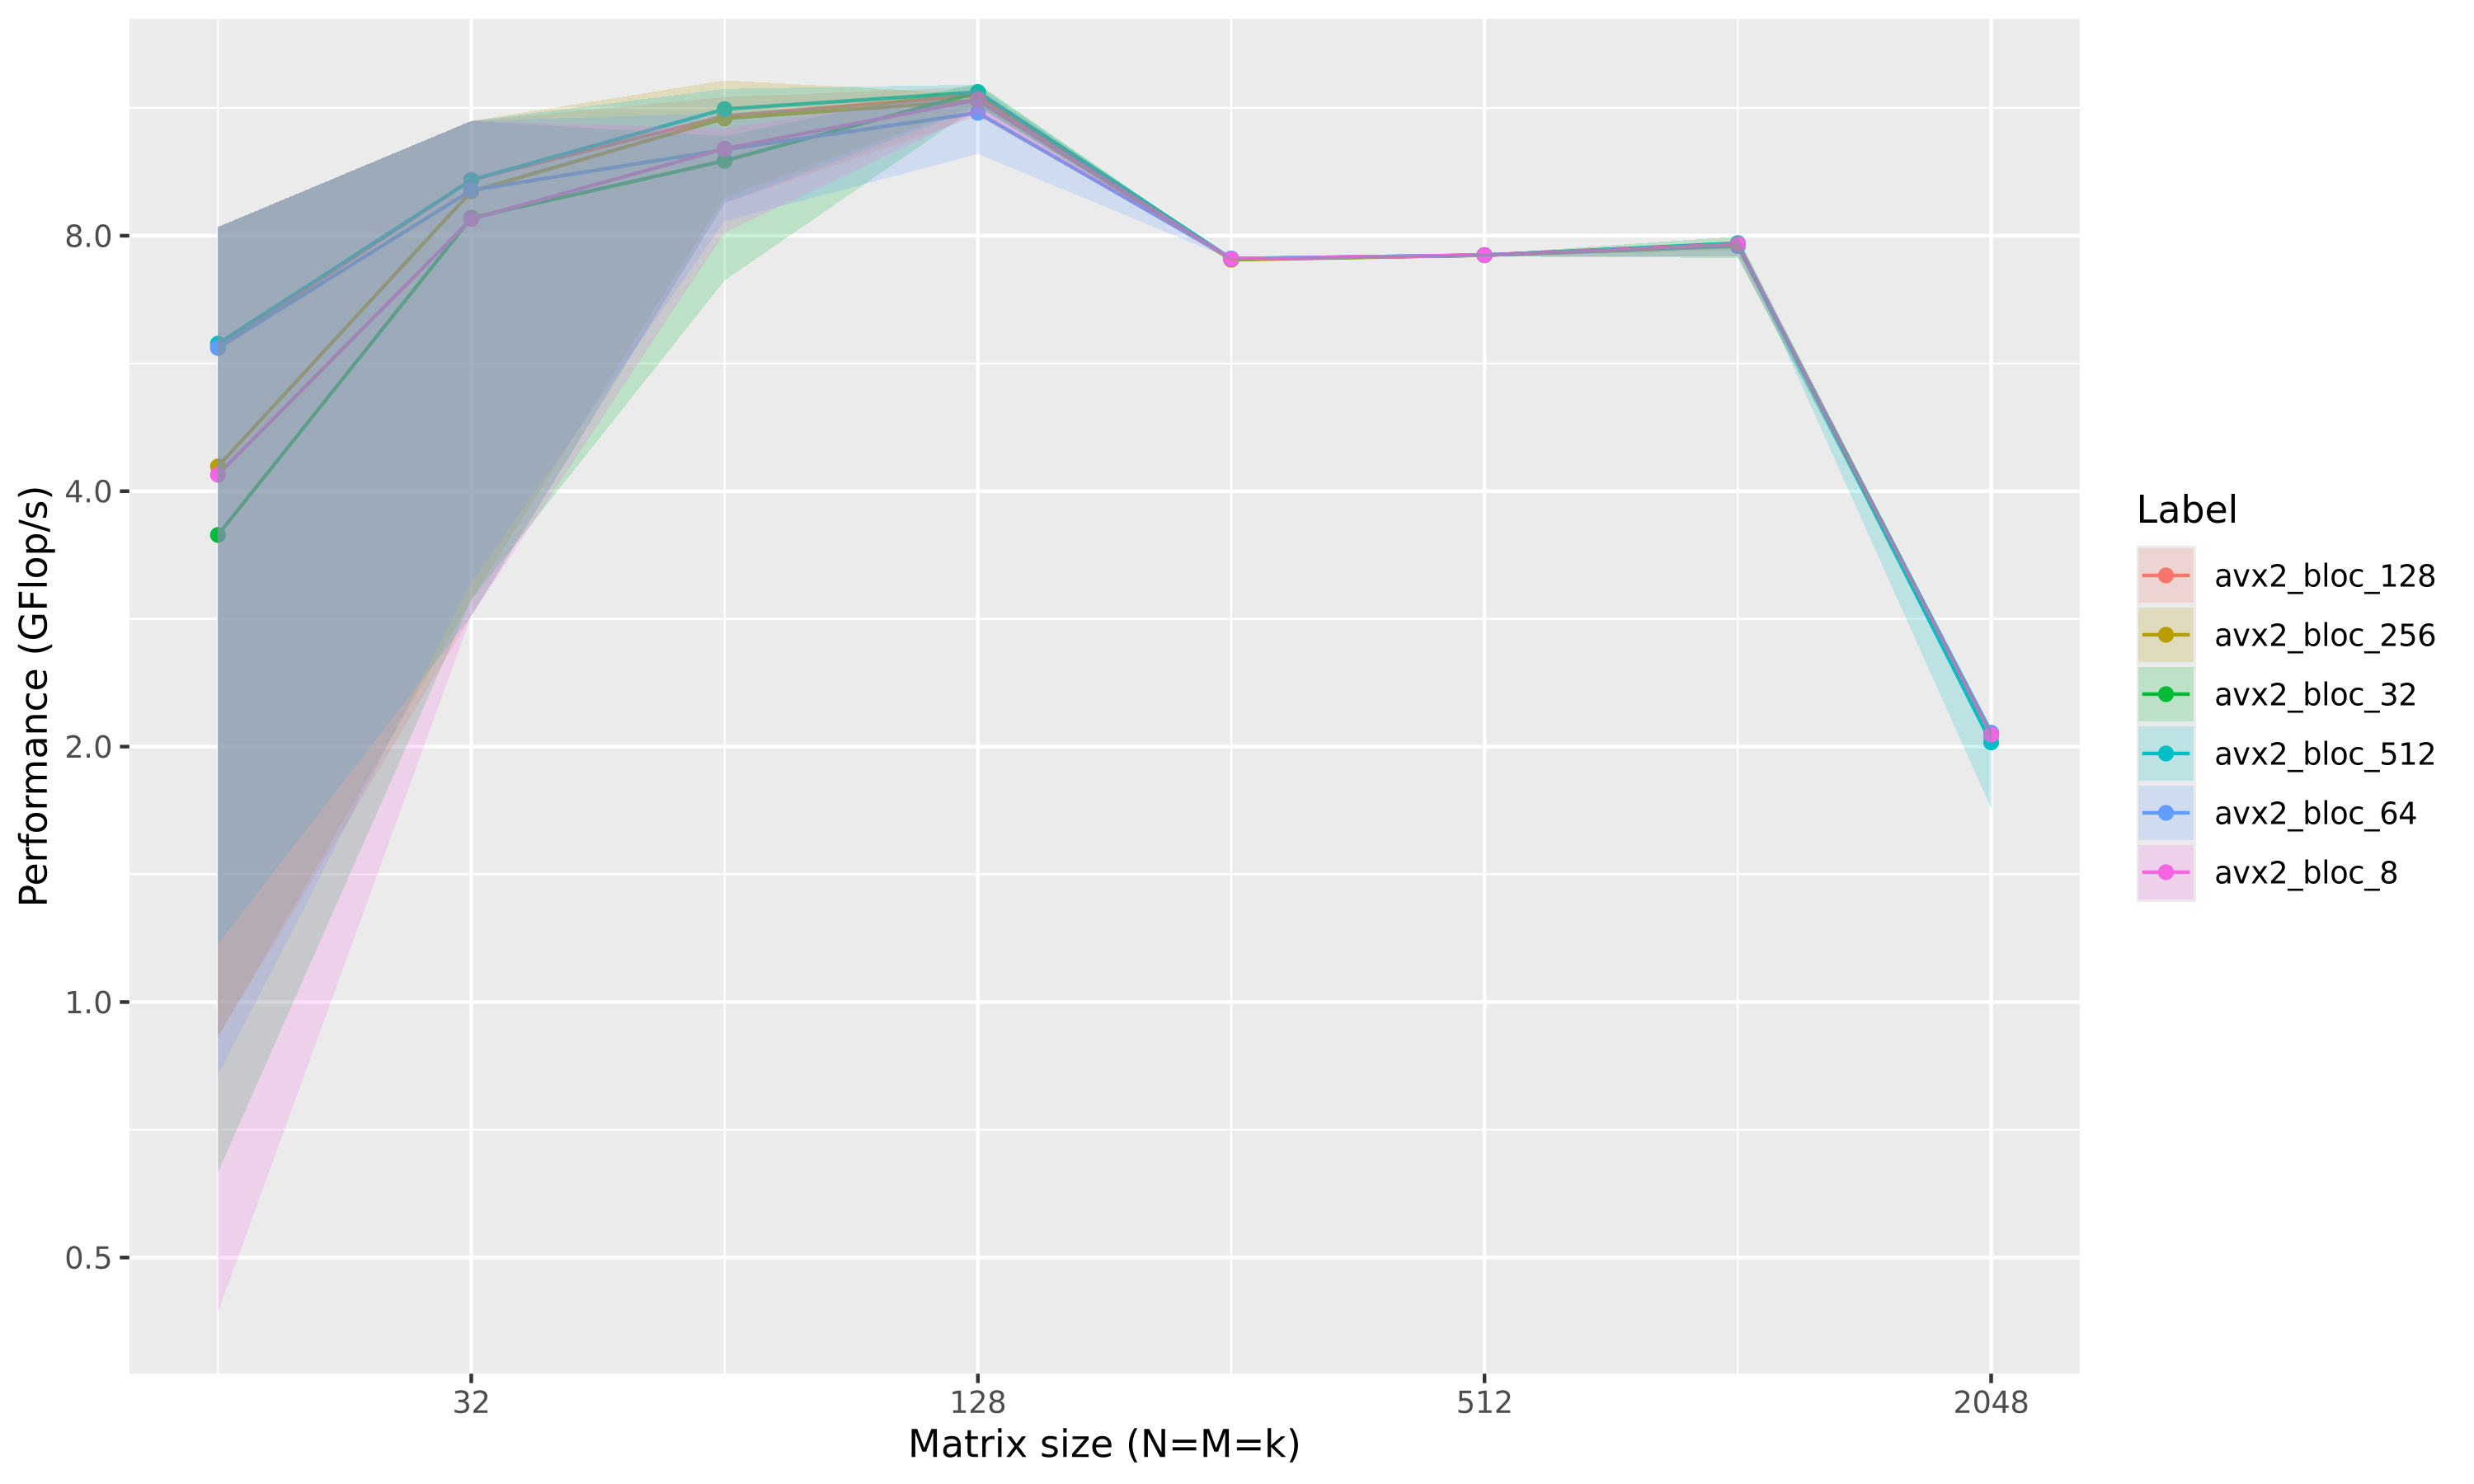
\includegraphics[width=1\linewidth]{assets/avx_bloc.png}
%     \caption{AVX2 + Blocage, différentes tailles de blocs}
%     \label{fig:placeholder}
% \end{figure}
% \subsection{Résultats}
% \begin{figure}[H]
%     \centering
%     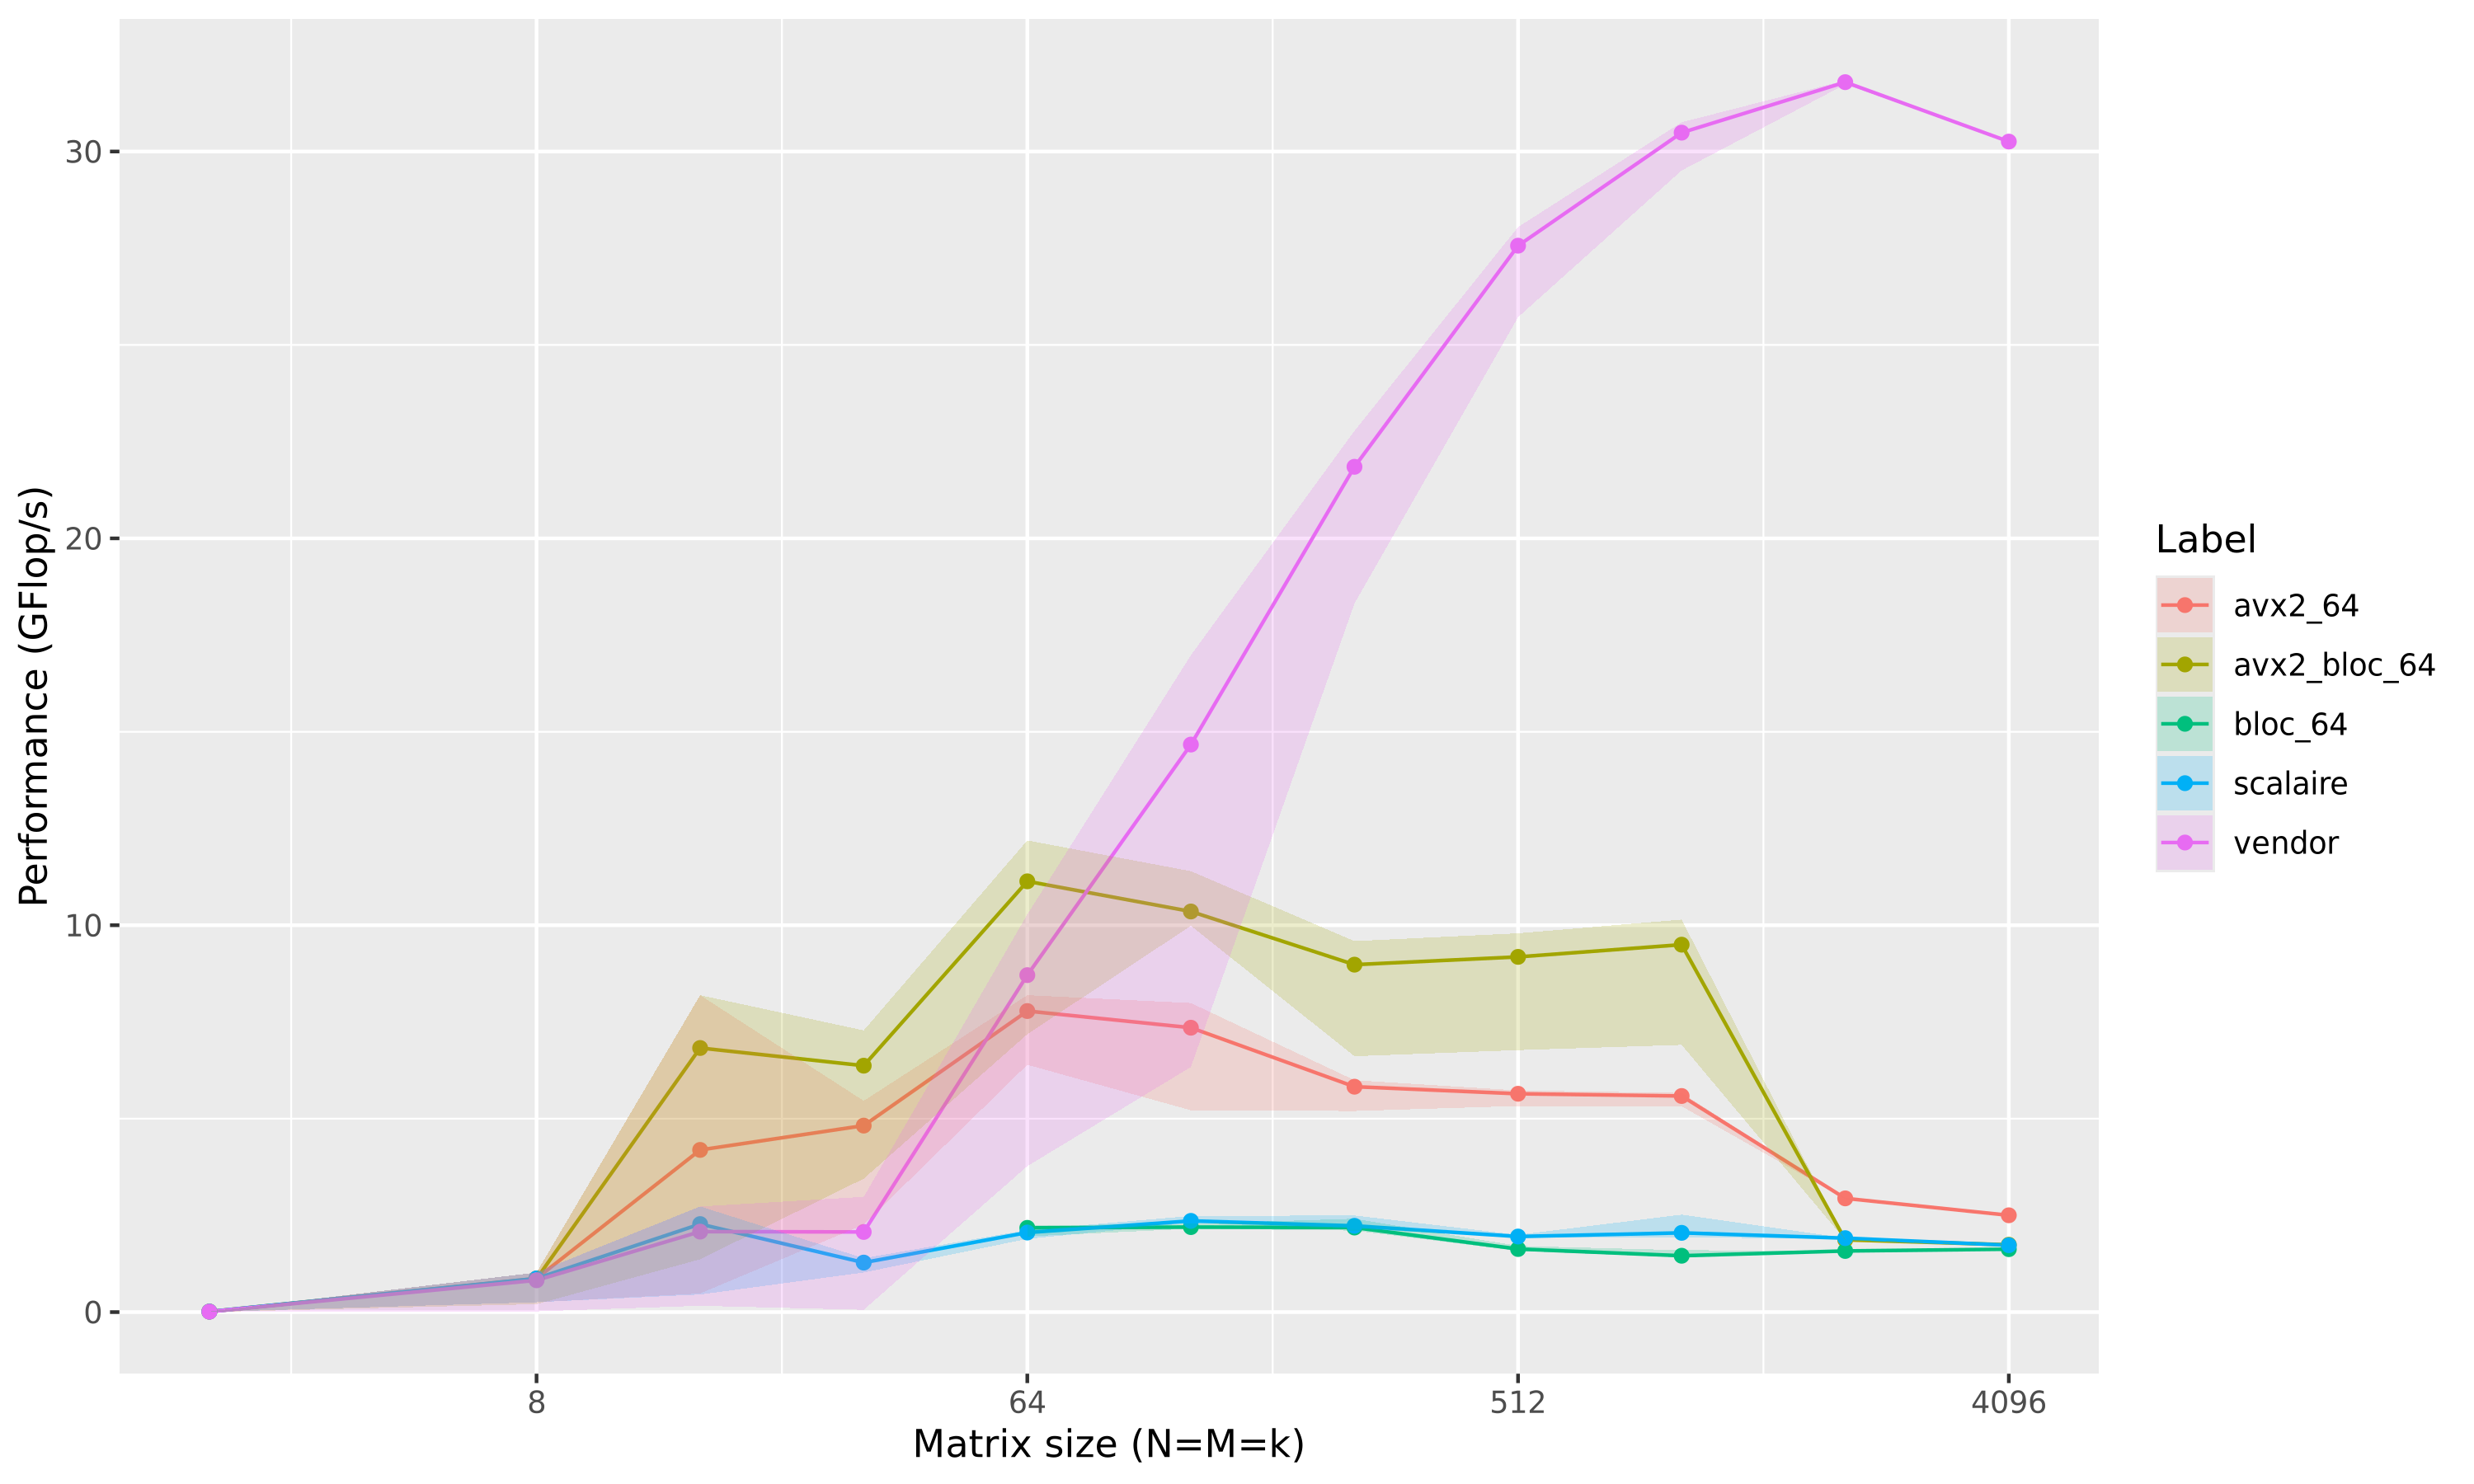
\includegraphics[width=1\linewidth]{assets/all_naive.png}
%     \caption{Comparaisons des performances des différentes versions séquentielles implémentées ainsi que de l'implémentation de référence (OpenBLAS)}
%     \label{fig:placeholder}
% \end{figure}

\section{Implémentation de l'article Anatomy of High-Performance Matrix
Multiplication}
\subsection{Avant Propos}
\begin{figure}[h]
    \centering
    \begin{minipage}{0.35\textwidth}
        Nous avons commencé par implémenter différentes versions séquentielles et AVX,
        bloquées ou non, avant de constater que les performances n'étaient pas au
        rendez-vous. Voici tout de même les performances observées pour les
        différentes versions, où l'on constate très clairement une très mauvaise
        gestion des caches et un effondrement rapide des performances.
    \end{minipage}
    \hfill
    \begin{minipage}{0.55\textwidth}
        \centering
        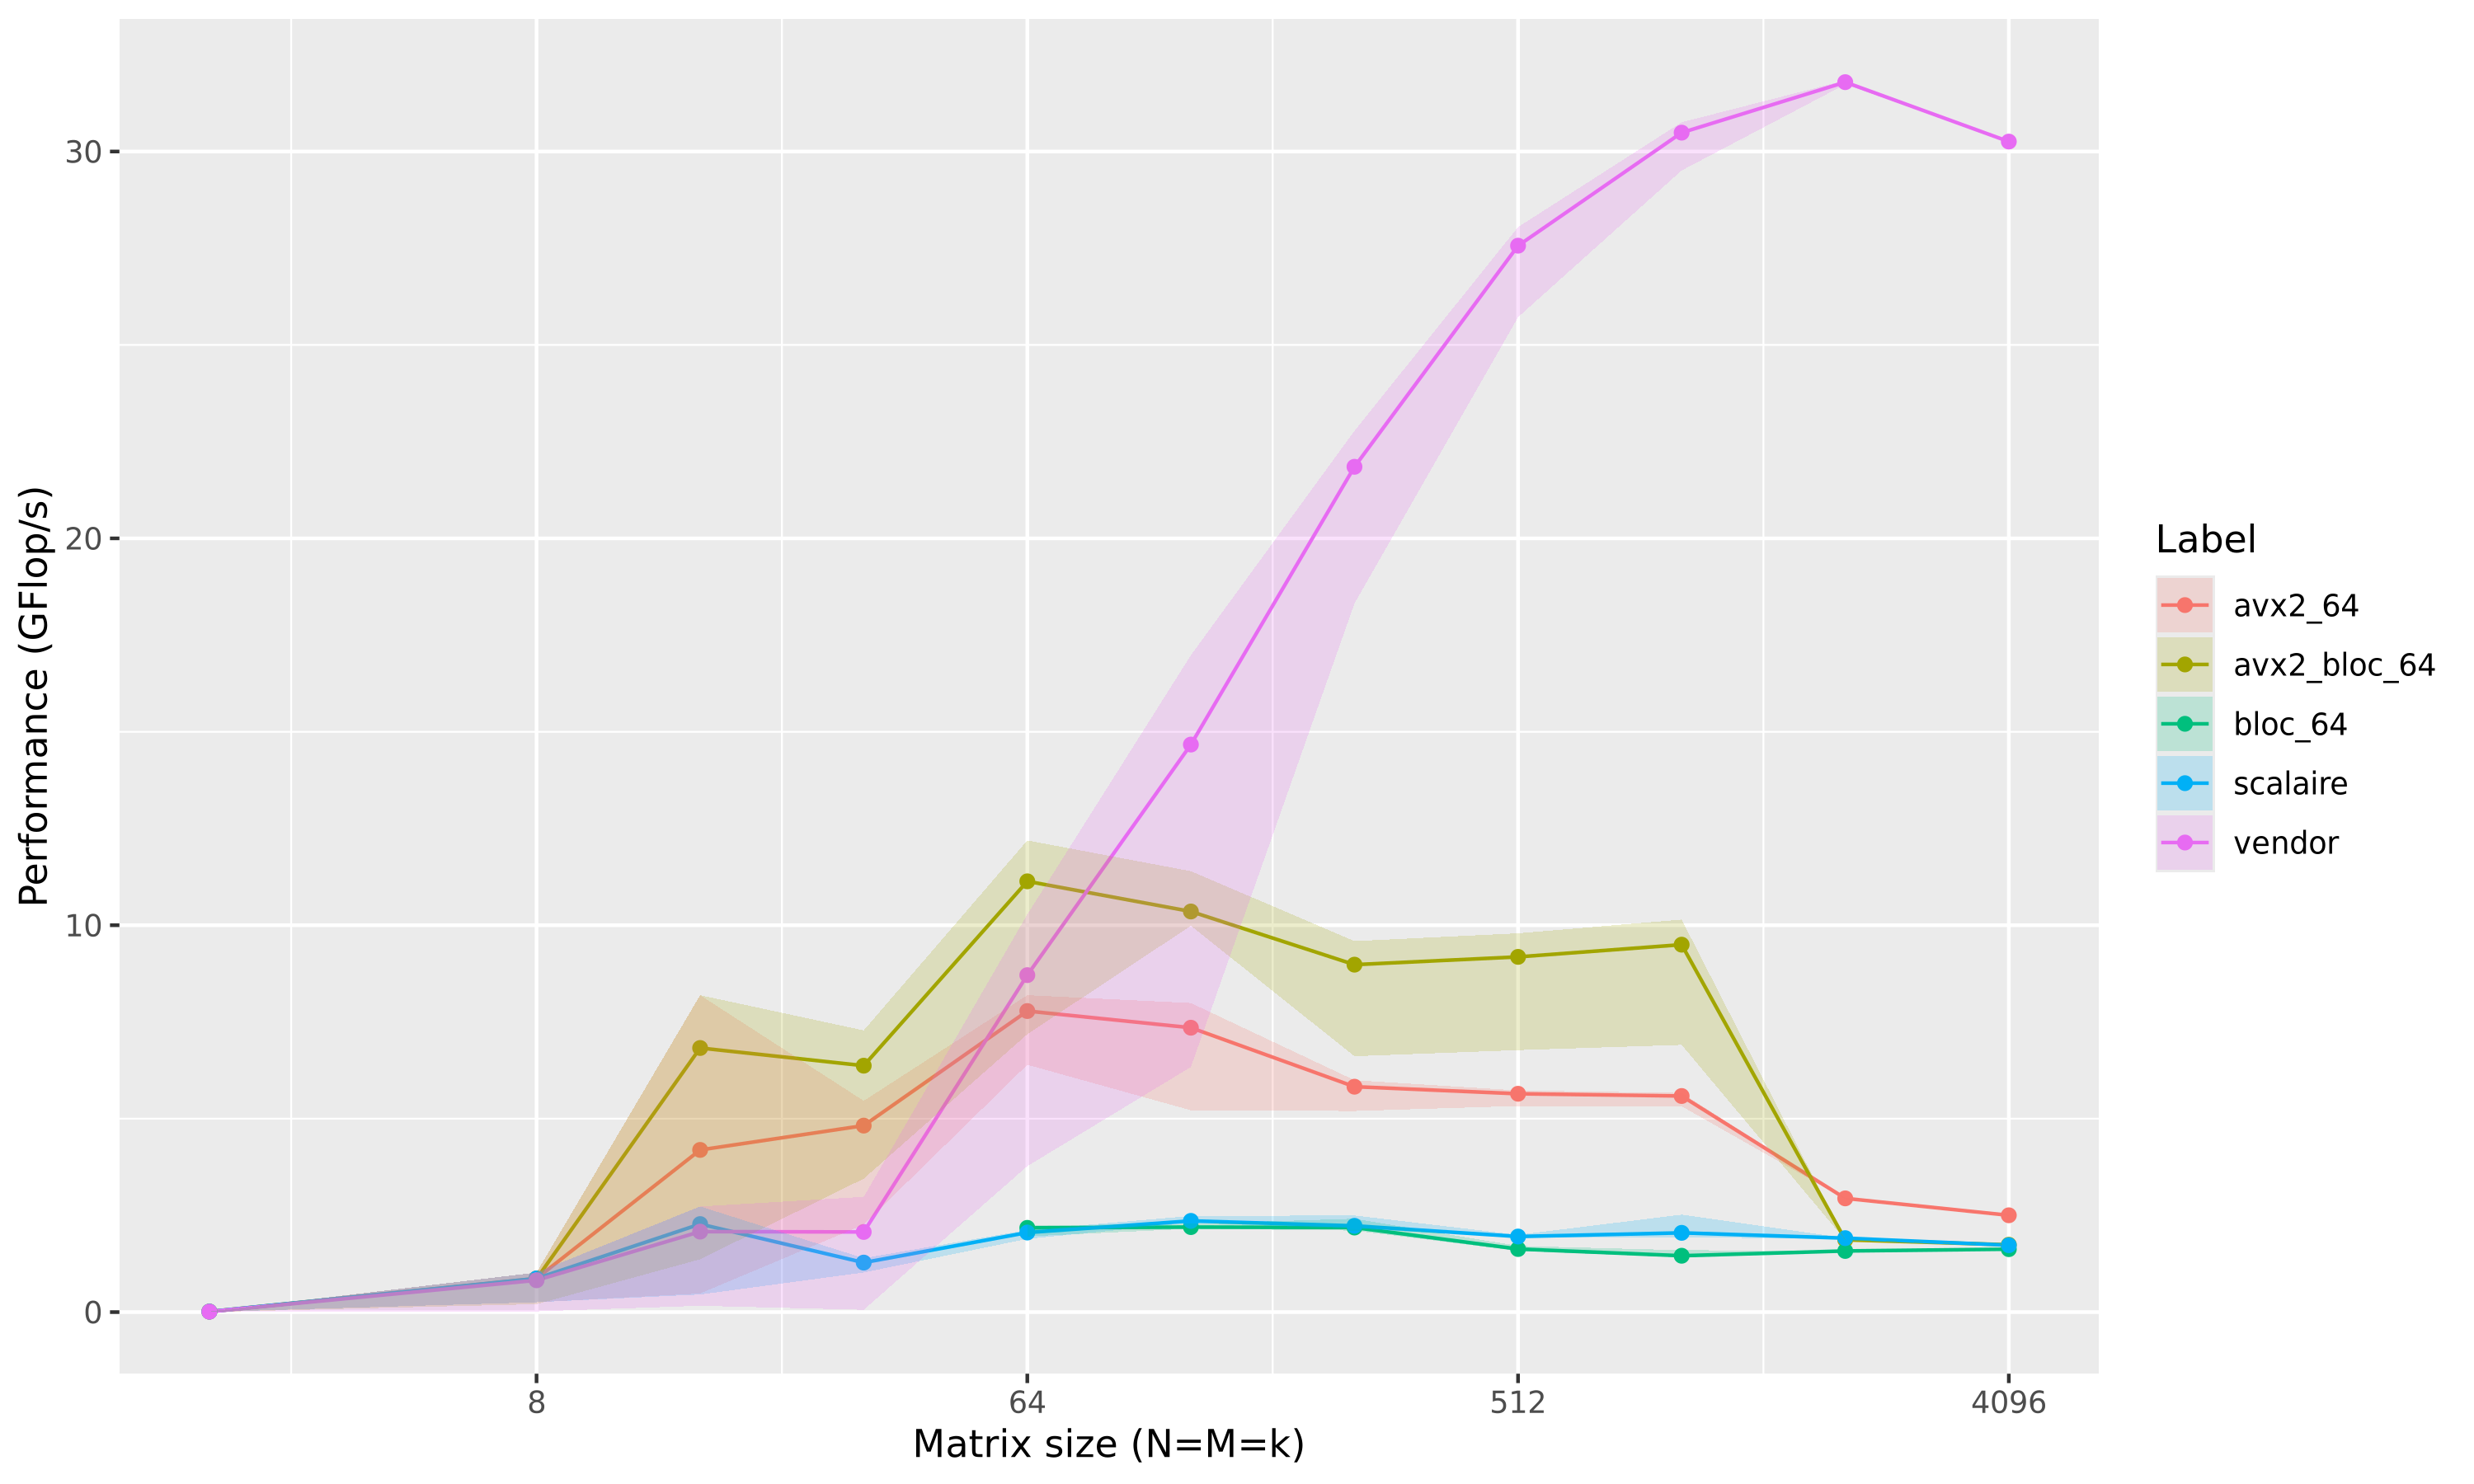
\includegraphics[width=\textwidth]{assets/all_naive.png}
        \caption{Comparaison des performances de nos premières implémentations, et de OpenBLAS (vendor)}
        \label{fig:perf_comparison}
    \end{minipage}
\end{figure}

\subsection{Idée générale}
Nous constatons que nous sommes bien loin du pic théorique même en utilisant le jeu d'instructions AVX et FMA, et que même sans viser ce pic nous restons loin de l'implémentation d'OpenBLAS ce qui signifie qu'il reste beaucoup de place à l'amélioration.\\
En cherchant des articles sur le sujet du GEMM séquentiel nous avons trouvé, entre autre, "Anatomy of High-Performance Matrix Multiplication"\cite{goto2008anatomy} qui propose un découpage des matrices à plusieurs niveaux afin de maximiser l'utilisation des caches. Il a également recours à de la réorganisation de la donnée dans des tableaux de travail afin de maximiser la contiguïté de ces dernières, en les ordonnant dans l'ordre de lecture du noyau de GEMM.\\

L'idée est de découper l'opération GEMM en plusieurs sous-problèmes plus petits et tenant dans les caches, à la manière d'un blocage classique. Un certain nombre d'approches sont présentées dans l'article, mais une seule est vraiment développée; c'est celle que nous avons tenté de comprendre et d'implémenter.\\

D'abord, nous découpons $A$ et $B$ en panels le long de la dimension de réduction $k$, panels de taille $KC$. Nous nous retrouvons désormais avec des panels de la forme $P_{A_i}\in\mathcal{M}_{M,KC}$ pour les panels de $A$, et $P_{B_i}\in\mathcal{M}_{KC,N}$ pour les panels de $B$ toujours dans le but de construire $C\in\mathcal{M}_{M,N}$.\\

Ensuite, nous appelons une opération GEPP (GEPanel x Panel). Dans cette opération, nous découpons le panel courant de $A$ en blocs la forme $B_{P_{A_i}}\in\mathcal{M}_{MC, KC}$, puis nous appellons une opération DGEBP (DGEBloc x Panel) avec le bloc courant de $A$ et le panel courant de $B$ qui a été préalablement réorganisé afin d'être contiguë sur la dimension $n$.\\

Finalement, DGEBP réorganise le panel de A en sous matrices de taille $MR\times NR$ avant  d'appeller un micro-kernel de taille $MR\times NR$ conçu pour tirer le meilleur parti de l'architecture du processeur.\\

Nous avons joint en annexe un schéma expliquant \ref{fig:goto-schema} l'algorithme avec une vue assez haut niveau.\\

L'intérêt de ce découpage est donc de faire en sorte de travailler avec des panels de $B$ et des blocks de $A$ ayant des tailles réduites et tenant dans les caches. De plus, la taille du micro-kernel dépend du nombre de registres disponibles par unité de calcul, ou plutôt du nombre de registres adressables par unité de calcul. Dans les faits, nous allons optimiser les paramètres afin de maximiser l'utilisation des registres sans en dépasser le nombre pour éviter au maximum les déchargements de registres sur le tas (register spilling).\\

\subsection{Choix des paramètres}
Nous avons la main sur un certain nombre de paramètres à savoir:
\begin{itemize}
    \item $MR$ et $NR$ la taille des blocs du micro-kernel.
    \item $KC$ et $MC$ la taille des dimensions $k$ et $m$ des blocs/panels.
    \item dans les faits, nous avons également un paramètre implicite $KR$. Le micro-kernel déroule la boucle de la réduction sur l'axe $k$, en les traitant par groupe de 8.
\end{itemize}

Bien que les étapes de réorganisation des données soient communes à toutes les architectures, le micro-kernel est quant à lui spécialisé pour utiliser efficacement ce qu'offre  l'architecture du CPU. Dans les faits, nous visons des processeurs d'architecture Haswell (Xeon E5-2680 v3, 2.50GHz, pic théorique de 40Gflop/s en double), offrant à l'usage 16 registres vectoriels. Sachant cela, nous avons décidé de fixer $MR=4$ et $NR=8$. Cela nous permet d'utiliser 8 registres vectoriels pour stocker les 8 colonnes de C, 1 registre pour stocker une ligne de A et 1 registre pour stocker un broadcast d'une valeur de B, pour un total de 10 registres utilisés. Nous avons également testé une configuration avec $MR=4$ et $NR=12$ dans le but de maximiser le nombre de registres utilisés mais les performances se sont dégradées. \\

Enfin, pour fixer KC et MC nous avons d'abord essayé de suivre les recommandations du papier, en fixant $KC=256$ et $MC=64$, puis avons expérimenté empiriquement en variant KC et MC pour finir avec $KC=256$, $MC=2048$. Ces valeurs devraient normalement sous-performer car $KC\ \times MC$ doubles dépasse largement les 256Ko du cache L2, mais nous supposons que c'est en parti du à un cache L3 assez large couplé au hardware prefetcher.

\subsection{Micro-kernel}
Nous nous focalisons sur le calcul Non Transposé x Non Transposé en Column Major.\\

En observant la sortie assembleur sur Godbolt \footnote{\href{https://godbolt.org/z/PPx1q9PYz}{Assembleur généré pour le micro-kernel, même version de GCC que sur PlaFRIM}}, nous constatons effectivement que l'on commence par charger les 8 colonnes de $C$, puis GCC déroule nos boucle préfixées par un \#pragma GCC unroll 8, en gérant l'éventuel résidu avec une table de branchement, et utilise bien les 10 registres ymm0-ymm9 prévus sans
les décharger sur le stack. La suite n'est qu'une succession de mov/broadcast/fmadd jusqu'à avoir parcouru l'entièreté de $K$, après quoi on saute au label de la sauvegarde des valeurs calculées dans C.\\

\subsection{Résultats}
Tout d'abord comparons cette version à OpenBLAS sur des matrices carrées, en lançant à chaque fois au moins 10 itérations par expérience:
\begin{figure}[H]
    \centering
    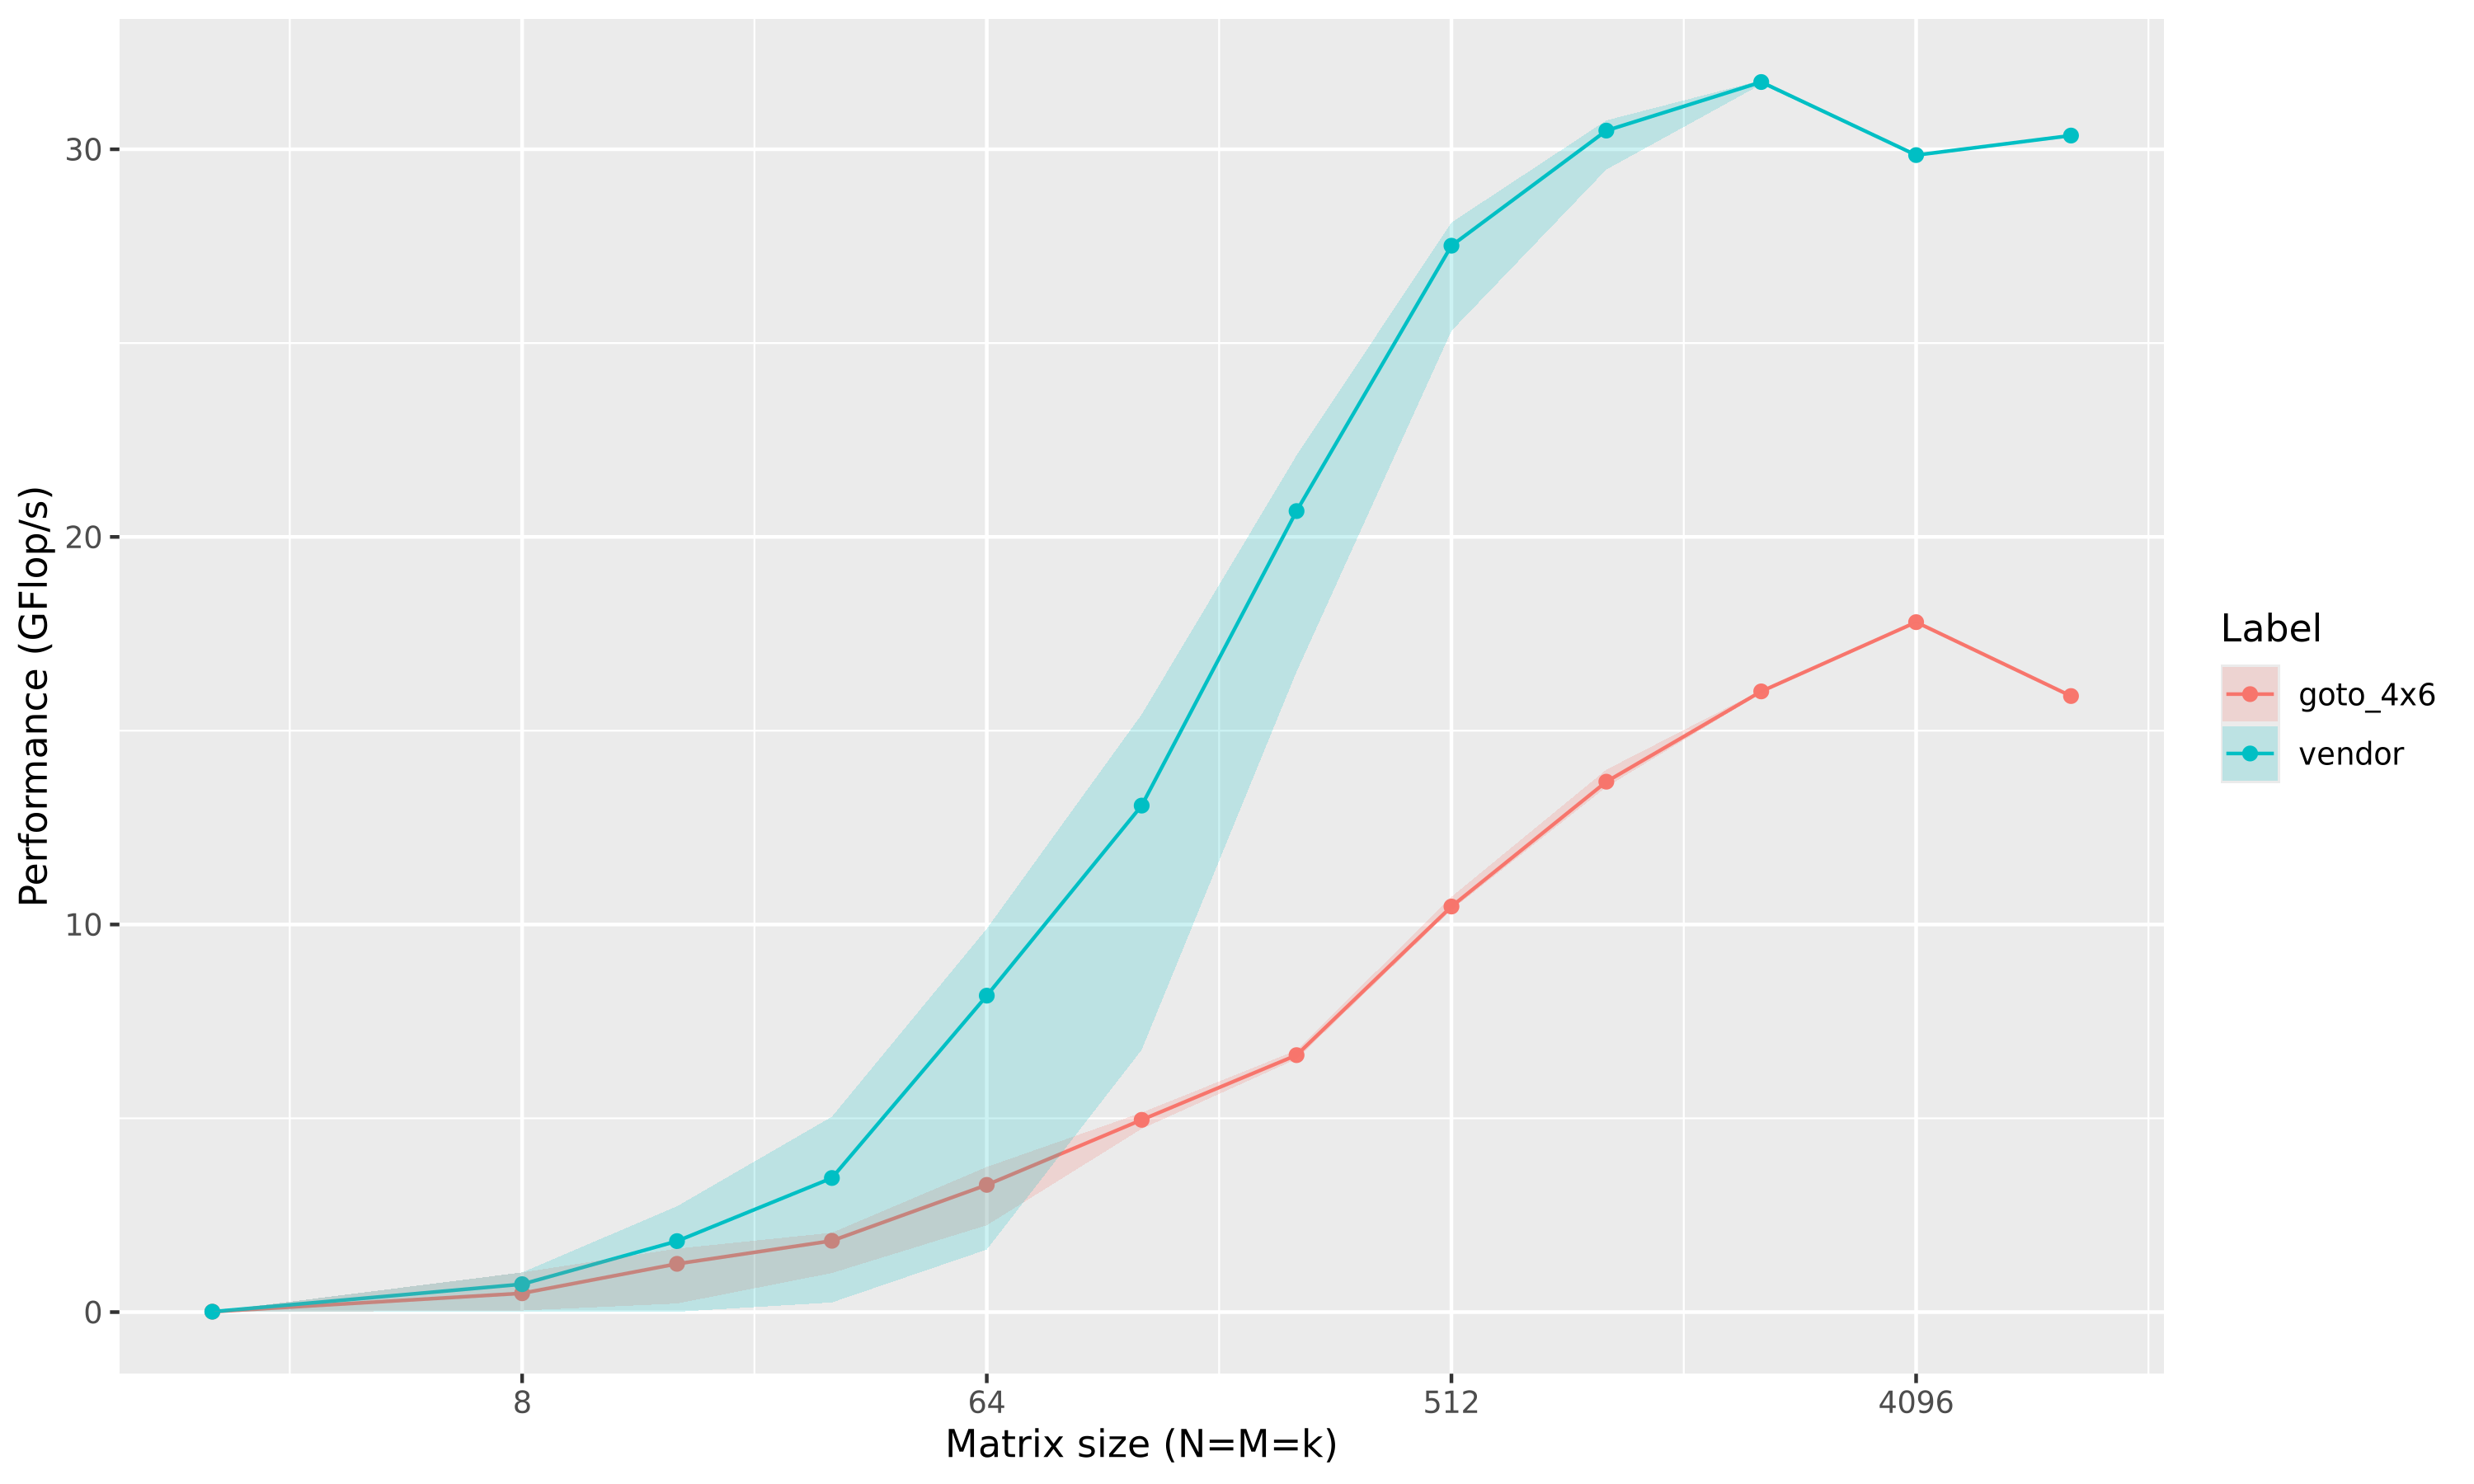
\includegraphics[width=.75\linewidth]{assets/vendor_vs_goto_square.png}
    \caption{Notre implémentation basée sur GOTO vs OpenBLAS}
    \label{fig:vendor-vs-seq-square}
\end{figure}

On voit bien qu'assez vite, OpenBLAS outreperforme notre implémentation, ce qui était attendu étant donné qu'il s'agit d'une évolution de GotoBLAS2. Cependant nous atteignons quand même en moyenne près de 75\% de ses performances. On constate également qu'une fois les matrices assez grandes pour maximiser l'intensité arithmétique (dans la mesure du possible pour un DGEMM), alors les performances restent constantes contrairement à nos premières tentatives de DGEMM qui finissaient toutes par avoir des chutes de performances dès lors que les matrices sortaient des caches.\\

Nous avons également décidé de faire la comparaison sur des combinaisons de tailles différentes pour les matrices en faisant varier indépendamment $M, N$ et $K$.
\begin{figure}[H]
    \centering
    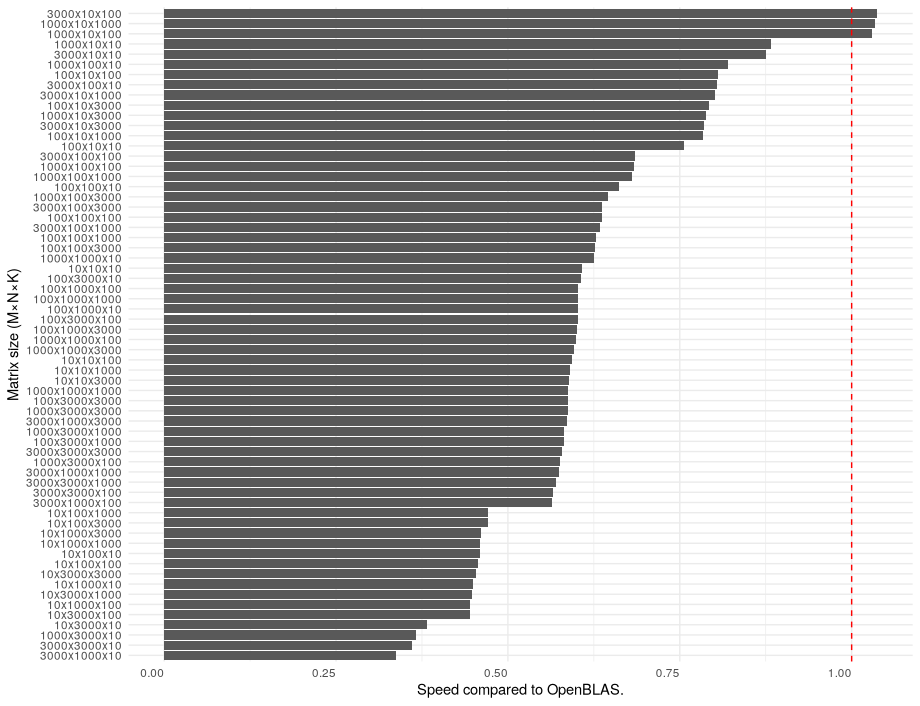
\includegraphics[width=.75\linewidth]{assets/vendor_vs_goto_diffsize.png}
    \caption{Comparaison entre notre implémentation GOTO et OpenBLAS sur différentes tailles de matrices}
    \label{fig:vendor-vs-goto-diffsize}
\end{figure}
Nous constatons que lorsque la dimension K est très petite, nous pouvons dépasser OpenBLAS même si les dimensions M et N sont grandes, avec par exemple 8192x8192x10, et c'est également le cas pour certaines configurations avec K=100. Cela tend à montrer que notre découpage est plutôt bon, et que c'est principalement le micro-kernel qui laisse place à de l'amélioration, même si c'est également dû à la simplicité de la prise de décision dans notre implémentation là où OpenBLAS a un surcoût dans le choix du chemin utilisé selon les caractéristiques de la matrice. En comparant les deux versions à l'aide d'Intel VTune nous constatons que nous saturons le pipeline de chargements depuis le cache L1 là où OpenBLAS semble moins limité par ce facteur. Nous supposons que cela résulte entre-autre d'un meilleur prefetching et d'un meilleur pipelining.
